\documentclass[12pt,a4paper, ngerman]{article}
\makeatletter
\def\set@curr@file#1{%
  \begingroup
    \escapechar\m@ne
    \xdef\@curr@file{\expandafter\string\csname #1\endcsname}%
  \endgroup
}
\def\quote@name#1{"\quote@@name#1\@gobble""}
\def\quote@@name#1"{#1\quote@@name}
\def\unquote@name#1{\quote@@name#1\@gobble"}
\makeatother
\usepackage{a4wide}
\usepackage{babel}
\usepackage{amsmath}
\usepackage[style=numeric]{biblatex}
\addbibresource{Maturarbeit.bib}
\usepackage{graphicx}
\usepackage{wrapfig}
\usepackage{listings}
\usepackage{xcolor}
\usepackage{xfrac}

\definecolor{codegreen}{rgb}{0,0.6,0}
\definecolor{codegray}{rgb}{0.5,0.5,0.5}
\definecolor{codepurple}{rgb}{0.58,0,0.82}
\definecolor{backcolour}{rgb}{0.95,0.95,0.92}
 
\lstdefinestyle{mystyle}{
    backgroundcolor=\color{backcolour},   
    commentstyle=\color{codegreen},
    keywordstyle=\color{magenta},
    numberstyle=\tiny\color{codegray},
    stringstyle=\color{codepurple},
    basicstyle=\ttfamily\footnotesize,
    breakatwhitespace=false,         
    breaklines=true,                 
    captionpos=b,                    
    keepspaces=true,                 
    numbers=left,                    
    numbersep=5pt,                  
    showspaces=false,                
    showstringspaces=false,
    showtabs=false,                  
    tabsize=2
}
 
\lstset{style=mystyle}

\begin{document}
\title{\large Maturitätsarbeit an der Kantonsschule Zürich Nord \\ \Huge Regelungstechnik \\ \huge PID-Parametrisierung anhand eines selbstgebauten Quadrocopters}
\date{\today}
\author{Charpoan Kong \\ M6d \\ Kantonsschule Zürich Nord}
\maketitle
\pagenumbering{gobble}





\newpage
\clearpage
\pagenumbering{Roman}
\tableofcontents
\newpage
\pagenumbering{arabic}

\section{Einleitung}
Ein Quadrocopter ist ein Flugobjekt mit vier Propellern. In der Vergangenheit wurden schon Versuche mit Flugobjekten mit vier Propellern gemacht z.B. wie der Luftfahrtpionier Étienne OEhmichen. der 1920 den Oehmichen No. 2 gebaut hatte. Damals waren die Propeller elastisch und man konnte mit Seilzügen den Anstellwinkel der Propeller einstellen. Er konnte damit einige Rekorde aufstellen.\cite{website:Wikipedia_Quadrocopter}\\ \\
In der heutigen Zeit finden Quadrocopter viele Anwendungen, wie z.B. bei Suchaktionen, im Militär, oder auch als Spielzeug. Mit der schnellen Entwicklung von Mikroprozessoren wurden Quadrocopter immer kleiner und einfacher zu realisieren. Auch können damit teurere Helikopterflüge für Kartographie oder Luftaufnahmen billiger realisiert werden.(Quelle)\\ \\
Die Intention zu dieser Arbeit folgt aus einem Projekt aus dem Freifachkurs Robotik. Damals kam der Raspberry Pi zum. Da der ein Betriebsystem parallel zum Flightcontroller am laufen hat, war die Regelung des Flightcontrollers zu träge. Desswegen wird auch ein neuer Chip evaluiert, der den Echtzeitanforderungen entspricht. \\ \\
\iffalse
Mit dieser Arbeit will ich mit dem Bau und dessen Regelung befasssen. Der Quadrocopter wird selbst gebau mit dem Hauptziel den Flightcontroller selbst zu designen, bauen und programmieren. So sollte die Regelung auch selbst implementiert werden. Dannach sollten Versuche gemacht werden, die bestimmen sollten, wie der PID-Regler stabiler gemacht werden kann und wie ungleichheiten, wie sie durch Vibration entstehen, auszugleichen. 
\fi
Die Fragestellung lautet, wie der die Regelung des Flightcontrollers implementiert werden muss, damit diese funktioniert und welche Faktoren diese stören und wie schnell die Daten verarbeitet werden müssen. Auch wird untersucht , welche Lösungen es für diese Probleme gibt und es wird cersucht diese zu implementieren. \\ \\
In der Arbeit wird der Quadrocopter selber gebaut, mit den Hauptziel den Flightcontroller selbst zu designen und zu programmieren. Dannach werden Versuche gemacht, die Bestimmten wie der PID-Regler stabiler gemacht wird und wie ungleichheiten, die durch Vibrationen enstehen, ausgeglichen werden können. Die Fernbedienung wird auch selbst gebaut und dient dazu Daten wärend des Fluges auszuwerten. 
\newpage
\section{Was ist ein Quadrocopter?}
Ein Qadrocopter ist wie in der Einleitung beschrieben ein Flugobjekt. Man könnte meinen, dass man einen stabilen Flug erreichen kann, wenn der Schub der vier Rotoren gleich ist. Aber dies ist leider nicht möglich, da viele Umwelteinflüsse einen stabilen Zustand verhindern wie z.B. Wind, unterschiede in den Rotoren oder Motoren, Assymetrie des Rahmens etc. So muss ein Computer, der Flightcontroller(FC), das Gleichgewicht erhalten, indem dieser den Schub der vier Motoren so reglelt, dass der Quadrocopter im Gleichgewicht ist oder dieser einen anderen bestimmten Winkel hält.\\
\begin{figure}[h]
\centering
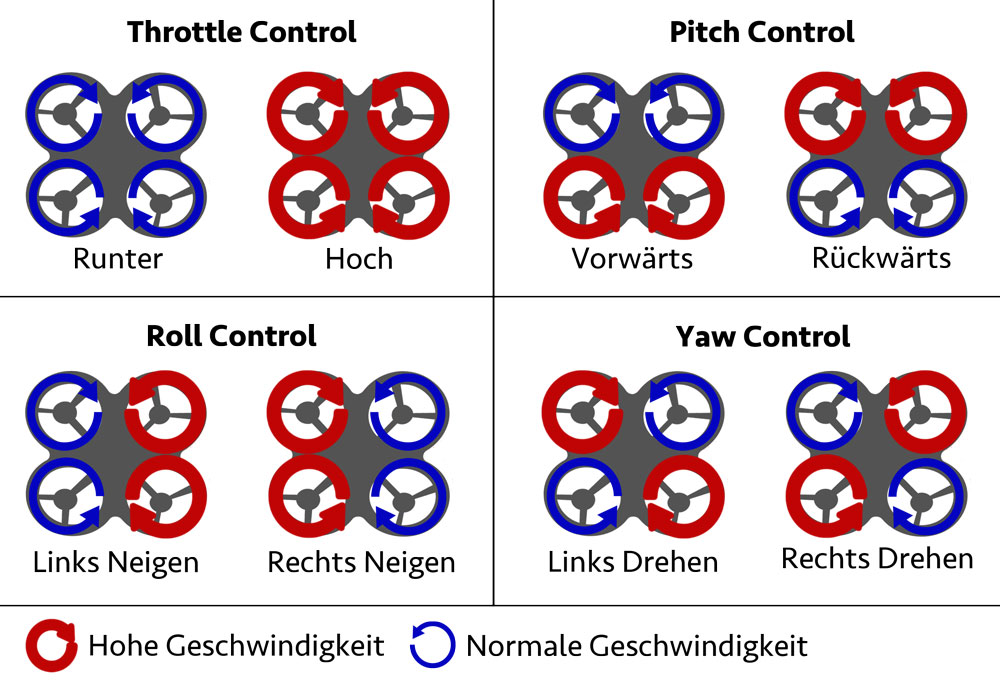
\includegraphics[width=\textwidth]{MotionDE.jpg}
\caption[https://fpvracing.ch/de/content/7-grundsatzliche-funktion-quadrocopter-multicopter]{Drehrichtung und Schub bei verschiedenen Steuereingaben }
\end{figure}\\
Abbildung 1 zeigt die Rotationsrichtung der Motoren gezeigt. Die benachbarten Motoren müssen eine gegensätzliche Rotation haben, da sonst der Quadrocopter ins Rotieren kommt. So wird das Drehmoment des anderen Motors ausgeglichen. Auch wird gezeigt, dass man den Quadrocopter mit erhöhen bzw. erniedrigen der Motorleistung der richtigen Motoren, diesen in die gewünschte Richtung steuern kann. Kernelement dieser Steuerung ist der PID-Regler.


\section{PID-Regler und Filter}
\subsection{Was ist ein Regler?}
Eine Regelung ist ein Steuerung mit Rückkoppelung. Es wird ein Wert z.B. die Drehzahl eines Motors überwacht und je nach gewünschter Drehzahl, das Drehmoment des Motors geregelt, dass er auch diesen halten kann, auch wenn eine Last am Motor hängt.\cite{website:rn-wissen_Regelungstechnik}\\
\begin{wrapfigure}[6]{r}{0.4\textwidth}
\centering
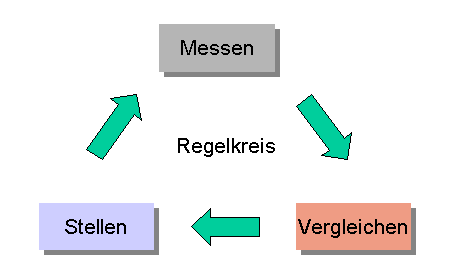
\includegraphics[width=0.4\textwidth]{Regelkreis1.png}
\caption[https://rn-wissen.de/wiki/images/2/25/Regelkreis1.png]{Der Regelkreis}
\end{wrapfigure}
Im Reglekreis wird der Ist-Wert z.B. mit einem Sensor gemessen. Dieser wird dieser mit dem Soll-Wert verglichen um die Regelabweichung zu bestimmen. So kann der Reglegrösse bestimmt werden um so das System dem Soll-Wert anzugleichen.\\ \\ \\ \\ \\ \\ \\
Die Regelabweichung kann dabei einfach mit der Differenz des Ist-Wertes $x$ mit dem Soll-Wertes $w$ bestimmt werden.\cite{website:rn-wissen_Regelungstechnik}
\begin{equation}
e(t)=w-x
\end{equation}\\

\begin{wrapfigure}[8]{l}{0.4\textwidth}
\centering
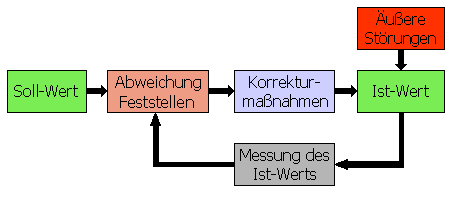
\includegraphics[width=0.4\textwidth]{Regelkreis2.png}
\caption[https://rn-wissen.de/wiki/images/5/5d/Regelkreis2.png]{Wirkungsweise des Regelkreises}
\end{wrapfigure}
In Abbildung 3 sieht man, wie vorher beschrieben, wie ein solcher Regelkreis funktionert. In der Regelungstechnik wird versucht einen solchen Regelkreis mathematisch zu modellieren. In diesem Kapitel wird nur der PID-Regler und seine Komponenten besprochen, da dieser häufig bei Quadrocoptern benutzt wird.(Quelle)\cite{website:rn-wissen_Regelungstechnik}
\\ \\ \\ \\
Der PID-Regler besteht aus mehreren Relgern und dem D-Glied. In der Folge wird beschrieben wie die einzelnen Komponenten wirken. 
\newpage
\subsubsection{P-Regler}
Der P-Regler wirkt linear. Dieser Regler gibt die Regelabweichung verstärkt und unverzögert mit dem Faktor $Kp$ weiter.(Vgl. \ref{p}) Das Problem dabei ist, dass diese Abweichung bleibend ist und somit den Soll-Wert über- bzw. unterschiesst. Dieser Regler wirkt mittelschnell.\cite{website:rn-wissen_Regelungstechnik}
\begin{equation}\label{p}
y(t)=Kp\cdot e(t)
\end{equation}

\subsubsection{I-Regler}
Beim Integralregler wird die Regelabweichung über die Zeit summiert und mit dem Faktor $Ki$ verstärkt.(Vgl. \ref{i}) Dabei werden Abweichungen volständig eliminiert, da dieser Regelwert immer anwächst solange die Regelabweichung nicht Null ist. Dieser Regler wirkt langsam.\cite{website:rn-wissen_Regelungstechnik}\\
\begin{equation}\label{i}
y(t)=Ki\int_{0}^{t}e(t)dt
\end{equation}

\subsubsection{D-Glied}
Das Differenzialglied schaut auf die Differenz der Regelabweichung zur vorherigen Regelabweichung und wird mit dem Faktor $Kd$ verstärkt.(Vgl. \ref{d}) Desshalb reagiert dieser sehr schnell und gibt den beiden anderen Vorhaltezeit.Differenzialglied ist kein Regler da es alleine nichts regleln kann sondern nur auf Veränderungen in der Regelabweichung reagiert.\cite{website:rn-wissen_Regelungstechnik}\\
\begin{equation}\label{d}
y(t)=Kd\cdot \dot{e}(t)
\end{equation}

\subsubsection{PID-Regler}
Beim PID-Regler werden die Eigenschaften der einzelnen Regler und dem D-Glied vereint.(Vgl. \ref{pid})
\begin{equation}\label{pid}
y(t)=Kp\cdot e(t)+Ki\int_{0}^{t}e(t)dt+Kd\cdot \dot{e}(t)
\end{equation}
\newpage
\subsection{Digitaler Low-Pass Filter}
Ein Low-Pass Filter filtert hohe Frequenzen heraus. Der Filter ist aus der Elektronik oder der Tontechnik bekannt. Beim Quadrocopter wird ein solcher Filter für das unterdrücken des Rauschens des Inertialsensors verwendet. Dieses Rauschen wird durch die Vibrationen der Motoren erzeugt und liegt ca. bei 133Hz.\\ \\
Beim vorliegenden Digitalen Low-Pass Filter (DLPF) wird ein analoger RC-Low-Pass Filter emuliert, wie der in Abbildung 4.\cite{website:Wikipedia_LPF}\\ \\
Im letzten Kapitel wurde der PID-Regler eingeführt, doch Vibrationen verursachen Störungen in der Regelung und führen so zu falschen korrekturen. Zum Beispiel verursachen Vibrationen beim D-Glied starke Auschläge, wenn diese hohe Amplituden haben. Auch wird dieser dann unbrauchbar, da die Regelabweichung durch die Vibrationen verfälscht wird. Ein Filter versucht diese Vibrationen zu dämpfen und verhindert so starke Ausschläge.
\begin{figure}[h]
\centering
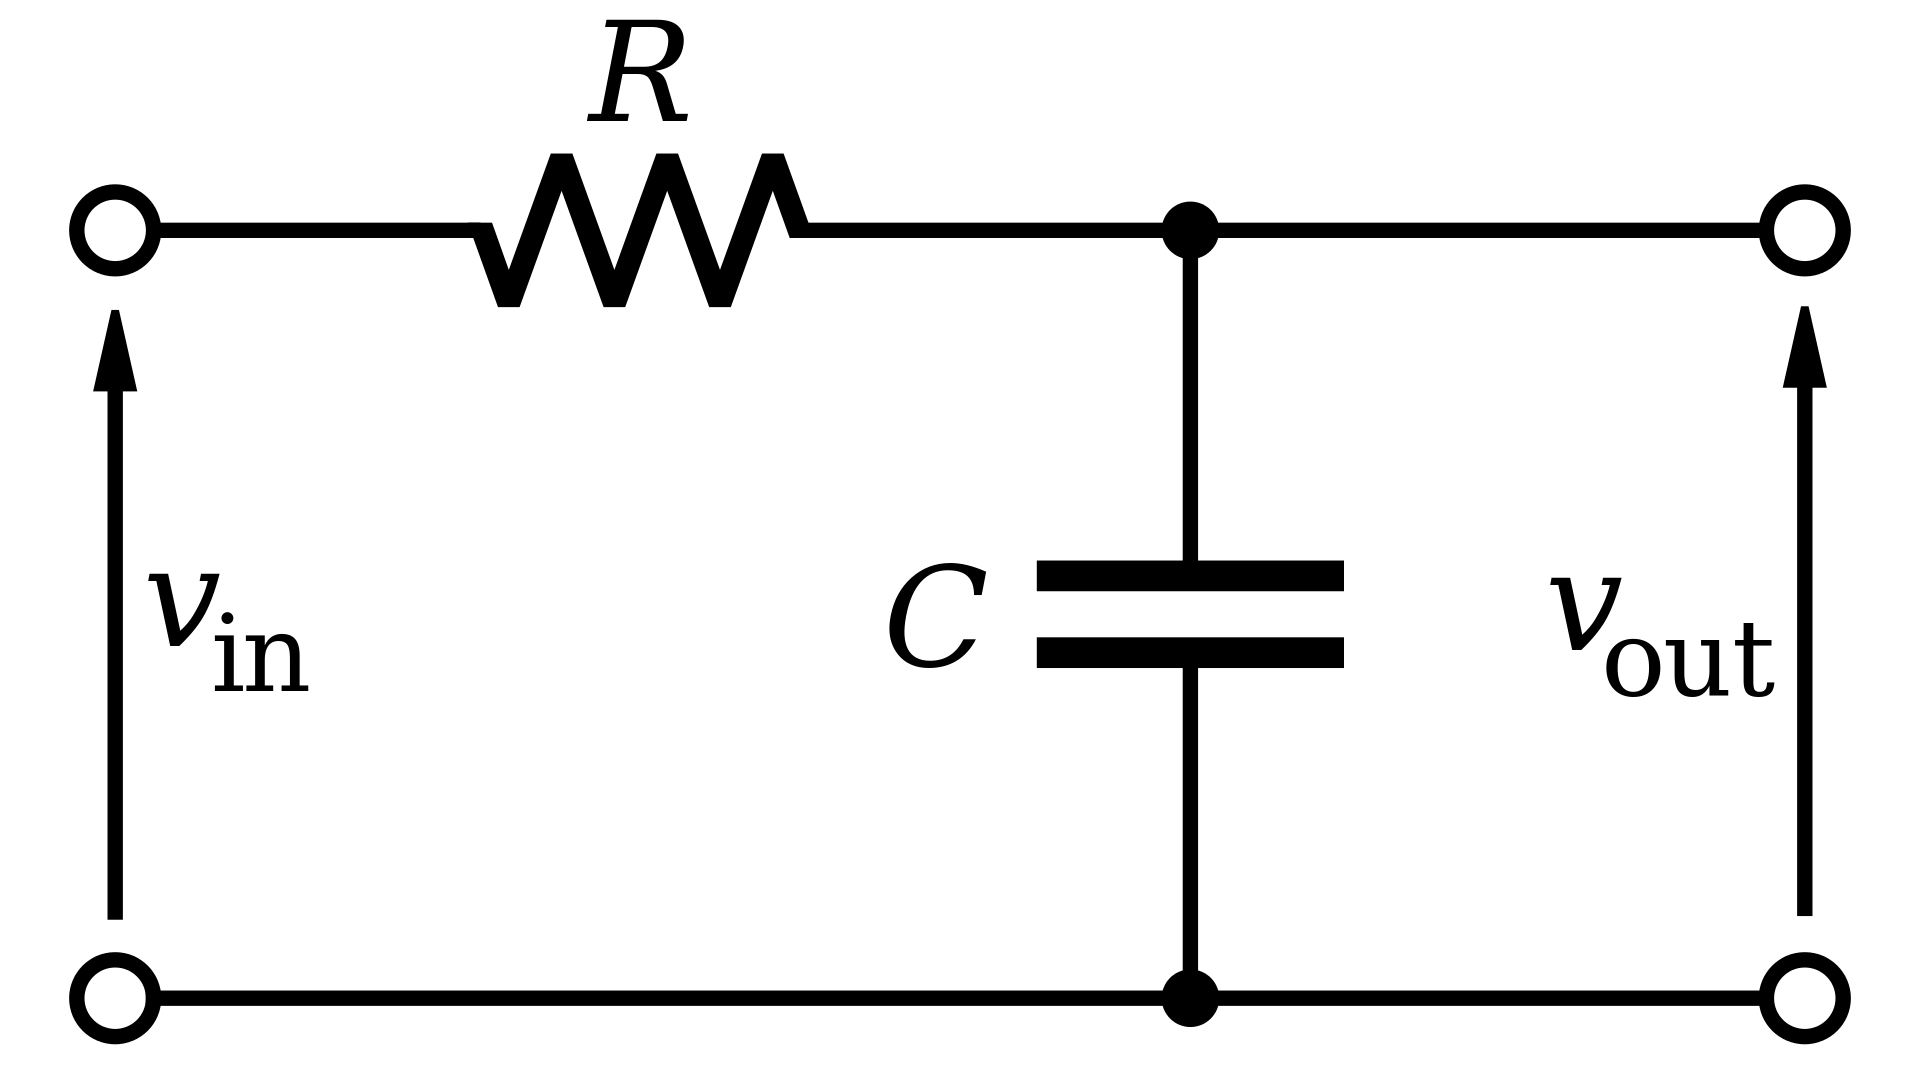
\includegraphics[width=0.4\textwidth]{DLPF1.png}
\caption[aasdf]{RC Low-Pass Filter}
\end{figure}\\
Wie man in \ref{eq1} sieht, ist die Eingang- und Ausgangsspannung vom Widerstand und von der Stromstärke abhängig.
\begin{equation} \label{eq1}
v_{\text{in}}(t)-v_{\text{out}}(t)=R\cdot I(t)
\end{equation}
Der Strom kann man auch abhängig vom Kondensator und der Ausgangsspannung darstellen wie man in \ref{eq2} und \ref{eq3} sieht.
\begin{equation} \label{eq2}
Q_{c}(t)=C\cdot v_{\text{out}}(t)
\end{equation}
\begin{equation} \label{eq3}
I(t)=\dot{Q}_{c}(t)=C\cdot \dot{v}_{\text{out}}(t)
\end{equation}
So kann man die Differenzialgleichung \ref{eq1} wie \ref{eq111} darstellen.\\
\begin{equation} \label{eq111}
v_{\text{in}}(t)-v_{\text{out}}(t)=RC\cdot \dot{v}_{\text{out}}(t)
\end{equation}
Jetzt wird $v_{\text{in}}(t)$ mit $x_{i}$ und $v_{\text{out}}$ mit $y_{i}$ dargestellt und die Differenzialgleichung diskretisiert zu der Differenzengleichung \ref{eq4}.
\begin{equation}\label{eq4}
x_{i}-y_{i}=RC\cdot \frac{y_{i}-y_{i-1}}{\Delta t}
\end{equation}
Die Gleichung \ref{eq6} (Ganze Auflösung siehe Anhang 1 Auflösung 1) wird nach $y_{i}$ umgeformt und man kann $\sfrac{\Delta t}{\Delta t+RC}$  mit $\alpha$ und $\sfrac{RC}{\Delta t + RC}$ mit $\alpha-1$ substituieren wie in \ref{eq5} gezeigt.
\begin{equation} \label{eq6}
y{i}=x_{i}\frac{\Delta t}{\Delta t+RC} + y_{i-1}\frac{RC}{\Delta t+RC}
\end{equation} 
\begin{equation}\label{eq5}
y{i}=\alpha x_{i} + (1-\alpha)y_{i-1} \quad \text{mit} \quad \alpha:=\frac{\Delta t}{\Delta t+RC}
\end{equation}
$RC$ kann mit der Formel für den Low-Pass Filter durch $f_{c}$ dargestellt werden wie unten gezeigt wird.
\begin{align*}
f_{c} = \frac{1}{2\pi RC} \\
RC = \frac{1}{2\pi f_{c}} 
\end{align*}
Jetzt kann auch das $RC$ in der Definition von $\alpha$ ersetzt werden, damit die Gleichung nicht mehr von $RC$ abhängig ist(Ganzer Beweis siehe Anhang 1 Beweis 1).
\begin{equation*}
\alpha = \frac{2\pi f_{c}\Delta t}{1+2\pi f_{c}\Delta t} 
\end{equation*}
\newpage
\section{Äusserer Aufbau}
\subsection{Motoren}
Die verwendeten Motoren sind sogenannte bürstenlose Motoren. Diese werden mit einem Electronic Speed Controller(ESC) angesteuert, dieser wandelt die Steuerimpulse in die richtige Spannung für den Motor. Da ihre RPM von Spannung abhängig ist, wird einen $Kv$-Wert angegeben. So kann man mit der Formel
\begin{equation}
a=Kv\cdot U \quad mit \quad a=[\text{rpm}]
\end{equation}
die Rotationen pro Minute berechnen.\\ \\
Beim vorliegenden Quadrocopter handelt es sich um ReadyToSky RS2205 Motoren mit einem $Kv$ von 2300. Diese Motoren wurden ausgesucht, da sie für genug Leistung bringen für einen Quadrocopter mit einer Rahmenlänge von 250mm.(Bild l)
\subsection{Akku}
Der Akku versorgt alle Komponenten, die Strom brauchen mit Strom. Im Quadrocopter wird ein LiPo Akku benutzt, der drei Zellen in Serie geschaltet hat mit einer Kapazität von 2.4Ah. Die miminale Spannung beträgt 11.1V. Die Entladerate wird $C$-Rate angegeben. Mit der Kapazität multipliziert wird der maximale Entladestrom ausgerechnet.\cite{website:fpvracing.ch_Mult_Komp}
\begin{equation}
I_{\text{max}}=Q\cdot C
\end{equation} (Bild r)\\ \\
Man benutzt in Quadrocoptern meist LiPo Akkus, da sie eine hohe Energiedichte besitzen und viel Leistung abgeben können. Dies aber hat auch zur Folge, dass man diese Akkus sorgfältig behandeln muss, da sie im Extremfall, Feuer fangen oder explodieren können. So darf man die einzelnen Zellen nicht unter einer Spannung von 2.7V fallen lassen. Desshalb wird der Akku auch an einem Akkuüberwacher angeschlossen, der piepst, wenn der Akku verbraucht ist. Auch braucht man ein Balanceladegerät, das kontrolliert, dass alle Zellen gleichmässug geladen werden. Eine hohe Kapazität garantiert nicht immer eine längere Flugzeit, da mehr Kapazität auch mehr Gewicht bedeutet.\cite{website:fpvracing.ch_Mult_Komp}
\newpage

\section{Der Flightcontroller}
Der Flightcontroller ist das Herz des Quadrocopter er liest alle Sensoren und gibt den ESCs die Steuerimpulse. In dem Kapitel wird zuerst in die wichtigsten Komponenten eingegangen, dann wird der Design-, Bau und Propgrammierprozess beschrieben.
\subsection{Komponenten}
\subsubsection{Microcontroller}
Der Microcontroller der auf dem FC benutzt wird ist ein ARM-Cortex-M7 STM32F722RET6 Microcontroller von STMicroelectronics. Dieser besitzt alle Schnittstellen um die einzelnen Sensoren und andere Komponenten auszulesen und anzusteuern. Da dieser nicht genug Pins hat, wird noch ein zweiter Microcontroller benutzt und zwar der ATMega328P, der auch auf dem Arduino/Genuino UNO zu finden ist. Dieser liest den Drucksensor und einige ADCs aus und kommuniziert mit dem I2C-Protokoll mit dem STM32. \\ \\
Microcontroller können anders als Mikroprozessoren, der auf dem Raspbery Pi verbaut ist, ohne Zusatz Pehpetrie benutzt werden, da sie schon einen Flash, RAM oder ähnliches. besitzen. Aber dies kommt mit einer tieferen Taktrate daher. Diese aber ist für den Quadrocopter völlig ausrreichend. Der Hauptcontroller lauft mit einer Taktfrequenz von 216MHz.

\subsubsection{Sensoren}
Die wichtigsten Sensoren des Quadrocopter sind der Gyrosensor und der Beschleunigungssensor. Der Gyrosensor misst die Winkelbeschleunigung der Achsen. In dem FC wurde eine ICM-20689 von TDK InvSense benutzt. Dieser hat beide Sensoren in einem Chip integriert und wird per SPI-Protokoll ausgelesen. Als Backup wird ein MPU-6050 benutzt, auch vom gleichen Hersteller, dieser wird mit dem langsameren I2C-Protokoll ausgelesen. \\
\begin{wrapfigure}[6]{r}{0.5\textwidth}
\centering
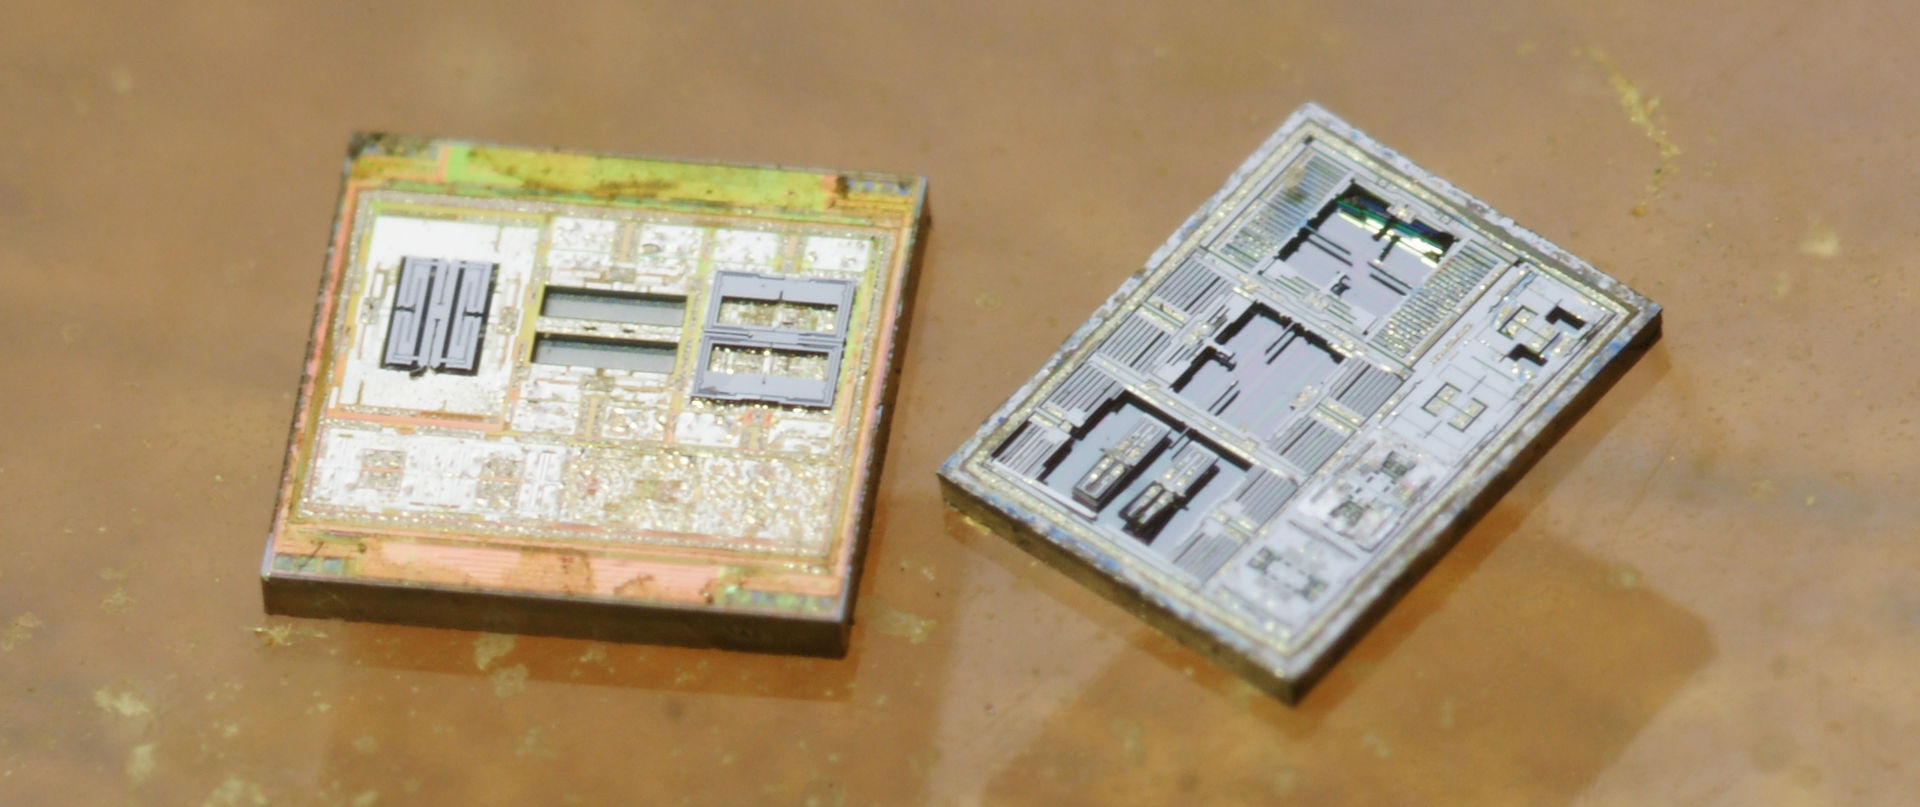
\includegraphics[width=0.5\textwidth]{1920px-Mpu6050-HD.jpg}
\caption[https://de.wikipedia.org/wiki/TDK]{Dice des MPU6050}
\end{wrapfigure}
Beide sind sogenannte MEMS-Sensoren. MEMS bedeutet microelectromechanical systems. Das bedeutet, dass diese Sensoren auf einer mechanischen Basis funktionieren.\cite{website:elek_Komp_MEMS}. Man ätzt die Sensorstrukturen und deren auslese Schaltung auf einen Chip.
\newpage
\noindent
Da der Gyrosensor nur Winkelgeschwindigkeit, bei den Sensoren $\frac{^\circ}{s}$ und nicht $\frac{rad}{s}$ misst muss diese noch mit der Loop-Zeit multipliziert werden um den Winkel zu bekommen.(vgl. \ref{aaa})
\begin{equation}\label{aaa}
w=\omega\cdot dt \quad mit \quad [w]=^\circ \quad und \quad [\omega]=\frac{^\circ}{s}
\end{equation}
Wenn man den Absoluten Winkel alleine mit dem Gyrosensor misst hat dieser über die Zeit einen Drift. Zum einen wird das durch das Rauschen im Sensor verurasacht und zu anderen auch von einem nicht genauen Loop-Zeit. Auch kann nicht der Anfangswinkel bestimmt werden und man müsste den Quadrocopter immer vom Boden aus starten. Deswegen braucht man da den Beschleunigungssensor. Dieser misst die Beschleunigung auf allen Achsen relativ zur Erdbeschleunigug. Beim Stillstand auf einer horizontalen Ebene misst er also
$
\begin{pmatrix}
0\\ 
0\\ 
1
\end{pmatrix}
\vec{g}
$. Man kann einfach die Norm des Beschleunigungsvektors $\vec{a} = \begin{pmatrix}
a_{x}\\ 
a_{y}\\ 
a_{z}
\end{pmatrix}$ nehmen und mit der Beschleunigung an der gewünschten Achse verrechnen um dann den Winkel zu bekommen.
\begin{equation}
w=\arcsin(\frac{a_{x/y}}{\vec{a}}
)
\vec{g}\cdot \frac{180}{\pi} \quad mit \quad [w]=^\circ
\end{equation}
Nebenbei muss man beachten, dass C/C++ den Winkel in $rad$ berechnet und man diesen noch zu $grad$ konvertieren muss. So hat man den absoluten Winkel mit zwei Sensoren gemessen und muss diese nur noch Kombinieren. Dies geschieht mit Hilfe des Komplementärflilters. (Man muss auch beachten das man nur den Absoluten Winkel nur für die Nick-und Rollachse berechnen kann da, für die Gierachse noch ein Magnetometer nötig wäre für eine Null-Referenz.)
\begin{equation}
w_{\text{komp}}=0.9996\cdot w_{\text{Gyro}}+0.0004\cdot w_{\text{Accl}} \quad mit \quad [w]=^\circ
\end{equation}
Dem Winkel aus dem Beschleunigungssensor wird ein tiefer Faktor gegeben da dieser Winkel nicht mehr genau stimmen wird, wenn der Quadrokopter in eine Richtung beschleunigen würde, dies wird erst bei starken Beschleunigungen der Fall sein, sonst stimmt dieser Wert ungefähr. Aber so kann man den Anfangswinkel des Quadrokopter bestimmen, ihn auch aus der Hand starten lassen und bekommt auch noch stabilere Werte. \\ \\
Desweiteren muss auch noch beachtet werden, das bei einer Bewegung um die Gierachse, der Sensor keine Bewegung auf der Roll- und Nickachse misst. Desshalb müssen die Werte dieser Achsen bei einer Bewegung um die Gierachse ineinander übersetzt werden mithilfe der Rotationsmatrix.
\begin{equation}
\binom{pitch'}{roll'}=\begin{pmatrix}
cos(\alpha) & -sin(\alpha)\\ 
sin(\alpha) & cos(\alpha)
\end{pmatrix}*\binom{pitch}{roll}
\end{equation}
Somit muss man die Achsen wie folgt verrechnen.
\begin{align} 
roll' = sin(\alpha)*pitch\\
pitch'= sin(\alpha)*roll
\end{align} 

\subsubsection{Empfänger}
Als Empfänger wir ein NRF24L01 Breakoutboard mit PA und LNA benutzt. Das ist ein 2.4GHz Sender und Empfänger der Firma Nordic Semiconductor. Die Kommunikation erfolgt digital und der Chip besitzt auch eine Zyklische Redundanzprüfung(CRC). Damit wird kontrolliert, ob ein Datenpaktet fehlerhafte Bits besitzt. Allenfalls wird es repariert oder verworfen. PA heisst Power Amplifying und bedeutet, dass das Signal verstärkt wird und so grössere Reichweiten erreicht werden können und LNA bedeutet Low Noise Amplifying und bedeutet, dass schwache Empfangssignale verstärkt werden.\cite{website:electronics.stackexchange.com_WhatisPALNA} Vom Hersteller wird eine Reichweite vom bis zu einem Kilometer versprochen aber in einer Wohnsiedlung kommt man mit Sichtkontakt bis zu 300m, was ausreichend ist.

\subsection{Leiterplatte}
Auf Leiterplatte oder auch Printed Circuit Board(PCB) wird die Schaltung des FC realisiert. Dieses besteht aus Kunststoff mit den aufgeätzten Kupferbahnen und den verzinnten Lötstellen.
\subsubsection{Design}
Zuerst habe ich mir überlegt was für einen Microcontroller ich wählen sollte. Bei meinen ersten Versuchen mit dem Raspberry gingen schief, da der Regler nicht schnell genug reagierte und eine nicht konstates Regelverhalten gezeigt hat. Einerseits lief ein Betriebsystem pararell zum Flightcontroller, adererseits war die Regelung nicht Echtzeit genug. Desswegen habe ich im Internet nachgeschaut was für Microcontroller auf den meisten Quadroopter verbaut sind. Dort werden  meist MCU aus der STM32-Familie verwendet. So kam ich auf die Webseite von Oscar Liang\footnote{\label{foot:1}https://oscarliang.com/f1-f3-f4-flight-controller/ aufgerufen am 31.03.2019} bei der die einzelnen MCU-Generationen aufgelistet waren mit den Vor-und Nachteilen. Ich entschied mich für die neuste Generation aus dieser MCU-Familie, einen STM32F7xx MCU zu benutzen. Nachher habe ich vorhandene Boards angschaut und gesehen, das die meisten den STM32F722RET6 benutzen aus dieser MCU-Generation. Als nächstes überlegte ich mir was für einen Gyro-und Beschleunigungssensor ich bentzen wolle. Ich habe schon eine MPU-6050 IMU aber ich wollte noch einen mit SPI-Protokoll, da dies schneller ist, und der andere als Backup, so recherchierte ich was für IMU's die FC's benutzen\footnote{\label{foot:2}https://blog.dronetrest.com/inertial-sensor-comparison-mpu6000-vs-mpu6050-vs-mpu6500-vs-icm20602/ aufgerufen am 31.03.2019} und entschied mich für den ICM-20689. Als Empfänger habe ich einen nRF24L01 PA + LNA gewählt.Als Backup wird noch ein PPM Eingang eingebaut für die standart Funkübertragung über eine normale Fernbedienung. Da für die Versuche Daten gebraucht werden, wird eine microSD-Karten Schnittstelle eingebaut, um die Daten aufzuzeichnen. Damit der Flightcontroller mit dem PC kommunizieren kann um zu Debuggen muss ein FTDI-Chip(F232RL) eingebaut werden damit wird das UART-Protokoll, in ein für den PC verständliches Protokoll übersetzt. Um die Höhe zu bestimmen habe ich mich für den BMP280 Drucksensor ausgewählt um die barometrische Höhe zu bestimmen. Da dieser für das auslesen eine lange Zeit braucht habe ich überlegt noch eine NebenMCU einzubauen. Deshalb habe ich den ATMega328 gewählt da er auch auf den Arduino UNO drauf ist und ich mich damit schon auskenne. Über diese MCU werden auch die Ultraschallsensoren ausgelesen, die eine genauere Höhenmessung ermöglicht, aber nur bis zu sechs Metern. Da die ESC's einen 5V Versorgungsausgang haben muss noch ein Spannungsregler  eigebaut werden, da die meisten IC's 3.3V braucchen, der Schulmechaniker Herr Thurnherr hat mir den LM3940 empfohlen.\\ \\
\begin{wrapfigure}[11]{r}{0.5\textwidth}
\centering
\includegraphics[width=0.4\textwidth]{egl.png}
\caption[Screenshot Eagle FC brd file]{Autodesk Eagle}
\end{wrapfigure}
Die Leiterplatte wird mit den Program Eagle von Autodesk designt. In dem Programm kann man die einzelnen Bauteile zusammensetzen und verbinden(Siehe Abbildung 5).Ich musste nach dem Datenblatt der einzelenen IC's, Konsendatoren und Wiederstände einbauen. Die Schaltbilder für die einzelnen IC's, die nicht schon in der Standartbibliothek vorhanden sind, habe ich aus dem Internet heruntergeladen. Herr Thurnherr hat mich dabei unterstützt und alle Fragen beantwortet. Nach mehreren Kontrollen wurde die Leiterplatte bei JLCPCB und die einzelenen Teile bei LCSC, Arrow, RS und Conrad bestellt. Dazu wurde noch eine Schablone für das SMD-löten bestellt. 

\subsubsection{Bau}
Beim Zusammensetzen des FC wird ein spezielles Lötverfahren gebraucht und zwar das SMD reflowing. Damit man die Komponenten nicht per Hand löten muss wird mit einer Schablone Lötpaste, die Flussmittel und das Lötzinn erhalten, aufgetragen. Dann wird die Schablone entfernt und die Teile werden plaziert. Dies geschieht im industriellen Rahmem mit sogenannten "Pick and Place" Maschienen. Später wird die Leiterplatte in den Ofen getan und nach einer bestimmten Temperaturkurve erhitzt, bis die Komponenten verlötet sind\cite{website:sauter-elektronik.de_reflow}.
\begin{figure}[h]
\centering
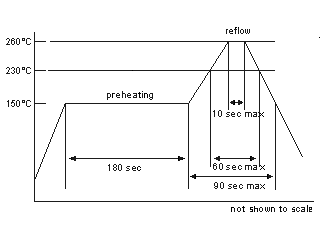
\includegraphics[width=0.4\textwidth]{reflow.png}
\caption[http://www.comtec-crystals.com/service-5.php]{Temperaturkurve für Reflowlöten}
\end{figure} \\
Da die Leiterplatte doppelseitig ist kann man hier nicht auf beiden Seiten das Reflow-Verfahren benutzen. Deshalb wurde Zuerst auf der Rückseite Lötpaste für den ATMega, dessen Quarzoszillator und dem SD-Kartenslot aufgetragen und die Komponenten wurden platziert. Dann wurden diese mit dem Heissluftföhn verlötet. Um das Herausfallen der Teile zu verhindern werden sie mit hitzebeständigen Klebeband fixiert.
Dann wurde auf einer Holzplatte Löcher an den Positionen der Verlöteten Komponenten gebohrt. Damit wird erreicht, dass man die Vorderseite, Plan auf dieser Holzplatte gelegt werden kann. Mit den restlichen PCBs, man kann nur fünf auf einmal bestellen, wurde ein Rahmen erstellt um so das teilweise gelötete Board zu fixieren. Dann wurde die Schablone ausgerichtet und festgemacht. So konnte man mit lötpaste und einem Spachtel die Löcher und somit auch die Lötstellen mit Lötpaste füllen. Dann wurde die Schablone entfernt. Mithilfe des Mikroskops wurden die Teile dann auf der Leiterplatte plaziert. Im Ofen wurden sie dann ungefähr nach der Temperaturkurve gebacken und so war die Vorderseite gelötet. Die Hinterseite wurden dann per Hand fertig gelötet worden. Dann wurden nur noch die Konnektoren angelötet und der Flightcontroller ist fertig zum programmieren.

\subsection{Programmierung}
Der FC wird mit C und C++ programmiert. Dabei wurde die STM32CubeIDE von STMicroelectronics benutzt, die eine Eclipse IDE mit den entsprechenden Bibliotheken vorinstalliert ist. Es wurden für die einzelnen Komponenten auch andere Bibliotheken benutzt, die z.t. umgeschrieben werden mussten für den STM32. Die Bibliothek für die IMU wurde aber selbst programmiert. Dabei kamen mehrere Probleme auf, z.b. das dass ChipSelect-Signal zu früh auf High ging.(Bild). In diesem Kapitel geht es um die grössten Hürden und wichtigsten Abläufe bei der programmierung des Quadrocopters. Im Listening 1 wird der grobe Ablaufplan des Programms gezeigt.

\begin{lstlisting}[language=C++,caption=Programmablauf Pseudocode]
int main(){
	initPID_Values();
	initPeriphial();
	initIMU();
	initnRF24();
	initSD();
	
	while(true){
		loop();
	}
	
	return 0;
}

void loop(){
	start = elapsedticks();
	
	calcTrueangle();
	writeSD() //every 200th loopcycle;
	calcError();
	calcPID();
	setMotor();
	
	stop = elapsedticks();
	looptime = stop - start;
}

void setMotor(){
	if(throttle < 100){
		motspeed[0:3] = 1024;	
	}else{
		motspeed[0] = throttle + roll + pitch + yaw; 
		motspeed[1]	= throttle + roll - pitch - yaw;
		motspeed[2]	= throttle - roll - pitch + yaw;
		motspeed[3]	= throttle - roll + pitch - yaw;
	}
	
	PWM_SET(M1, motspeed[0]);
	PWM_SET(M2, motspeed[1]);
	PWM_SET(M3, motspeed[2]);
	PWM_SET(M4, motspeed[3]);
}
\end{lstlisting}

Die IMU und der Empfänger werden per Interrupt ausgelesen. Die  IMU gibt im 1KHz Takt ein Interruptsignal , dass beim lesen dann zurückgesetzt wird. Beim Empfänger wird ein Interruptsignal ausgegeben sobald neue Daten vorhanden sind.

\subsubsection{Motoren und Timing}
Die ESC's der Motoren müssen mit dem OneShot125 Protokoll\cite{website:OL_OneShot125} angesprochen werden. Bei dem wird ein PWM-Signal von 2khz erzeugt. Der Nullpunkt, bei dem die Motoren aus sind, liegt bei einer Periode von 125us bzw. einem PWM von 25$\%$. Die Motoren erreichen ihre maximale Drehzal bei einer Periode von 500us bzw. bei einem PWM von 50$\%$. (Bild).
\subsubsection{PID Implementierung}
Der PID-Regler wird für den absoluten Winkel und für die Winkelgeschwindigkeit implementiert, wobei man die Gierachse nur mit der Winkelgeschwindikeit implementieren kann, da keine Referenz besteht, z.b durch ein Magnetometer. Die Regelungsdifferenz und Regelungskorrektur wird jeden Loop-Zyklus berechnet mit ca 2kHz.

\section{Fernbedienung}
Die Fernbedienung wird aus Holz und PLA gebaut. Der Rahmen wurde mittels eines 3D-Drucker gedrukt.(Bild) Das Frontpanel ist aus Holz gelasert worden. Die Schieberegler wurden aus einer kaputten Fernbedienung genommen. Auch besitzt diese ein LCD-CharDisplay mit 20x4 Zeichen. Dies wird benutzt um den genauen Ausschlag der Schieberegler, die Sensorwerte und die PID-Werte anzuzeigen bzw. zu bearbeiten. Als Microcontroller wird ein STM32F767ZI benutzt der auf einem Nucleo-144 Protoboard verbaut ist. Listening 2 zeigt den Ablaufplan des Programmes.
\begin{lstlisting}[language=C++,caption=Programmablauf Pseudocode]
int main(){
	initPeriphial();
	initADC();
	initnRF24();

	while(true){
		loop();
	}
	
	return 0;
}

void loop(){
	readADC();
	sendData();
	
	menu_print();
}

void menu_print(){
	MENU_1:
		print_ADC_VAL();
	MENU_2:
		print_ACK_VAL();
	MENU_3:
		print_PID_ROLL_PITCH(); //<-- ALSO EDIT VALUES ON 0% Throttle
	MENU_4:
		print_PID_YAW(); //<-- ALSO EDIT VALUES ON 0% Throttle
}


\end{lstlisting}
\newpage

\section{Versuche}
Nach dem Bau des Quadrocopter und der Fernbedienung wurden tests in der Turnhalle der Schule gemacht, da der Quadrocopter schwerer ist als 0.5kg und dies gegen die Bestimmungen des Bundesamtes für Zivilluftfahrt ware(Quelle). \\ \\Zuerst wurden Versuche gemacht um den richtigen Wert des P-Reglers, der Nick- und Rollachse zu bestimmen. Der Wert wurde so lange erhöht, bis der Quadrocopter zu oszillieren begann. Dann wurde er in die Mitte der Turnhalle gestellt und es wurde der erste Flug probiert, der auch gescheitert ist. Es wurde dann auch probiert das D-Glied einzustellen, aber diese sind auch gescheitert. Später bemerkte ich den Fehler mit dem übersetzen der Winkel, der im Kapitel über den Inertialsensor, beschrieben wird. Als dieser Verbessert wurde, war das Verhalten des Quadrocopters immmer noch nicht befriedigend und dieser regelte immer noch zu schwach. \\ \\ Desshalb wurde das Verhalten des Quadrocopters mit einer funkionierenden Quadrocopters des Mechaniker verglichen. Dadurch wurde sichtbar das die Oszillation des P-Reglers gar nicht zu stark war sondern sogar viel zu schwach. Also wurden Versuche gemacht bei dem der P-Regler um das fünffache vergrösstert worden ist und ein D-Glied gesetzt, das ein zehntel des P-Reglers entsprach. Diese Versuch war dann erfolgreich und der Quadrocopter machte einen unstabilen oszillierenden Flug. Dennoch sah man das der Flightcontroller richtig regelte. \\ \\
Zurück zu den ersten Versuchen. Bei der Gierachse wurde auch zuerst ein P-Regler Wert eingesetzt. Aber diese korrekturen führten immer zu einem Purzelbaum des Quadrocopters. Aber der Mechaniker hat dann gesagt, dass die Gierachse mit ca. 5 Hz läuft. So wurde auch der obengenannte Digitale Lowpass-Filter einprogrammiert, der die Werte der Gierachse auf 5 Hz filtert. Auch wurde ein kleines Python Programm geschrieben, der die aufgezeichneten Sensor Werte filtert und so die Effekte des Filters sichtbar wurden. Man muss dabei beachten, dass das Verhalten des Flightcontrollers nicht damit dargestellt werden konnen, da er die Werte noch ungefiltert verarbeitet hat. Dennoch waren die darrauffolgenden Versuche nicht erfolgreich. So wurde das Augenmerk zuerst auf die Nick- und Rollachse geworfen. \\ \\
Beim leztzen Versuch ist es leider zu einem Unfall gekommen und einer der Motoren wurde beschädigt somit kann auch die Versuchsreihe bis zur Abgabe der Maturarbeit nicht weitergeführt werden, da die Motoren eine lange Lieferfrist haben und auch ein neuer Rahmen von Vorteil ist, da beim alten die Beine beschädigt waren und nicht richtig repariert werden konnten. Somit ist der Quadrocopter bis zur Abgabe noch nicht flugfähig.
\newpage

\section{Schlussfolgerung}

\newpage
\section{Quellenverzeichnis}
\subsection{Literaturverzeichnis}
\printbibliography
\subsection{Abbildungsverzeichnis}
\listoffigures
\newpage
\section{Anhang 1}
Auflösung 1:
\begin{align*} 
x_{i}-y_{i}&=RC\cdot \frac{y_{i}-y_{i-1}}{\Delta t} \\ 
x_{i}-y_{i}&=\frac{RCy_{i}-RCy_{i-1}}{\Delta t}\\
x_{i}\Delta t-y_{i}\Delta&=RCy_{i}-RCy_{i-1} \\
y_{i}\Delta t+RCy_{i}&=x_{i}\Delta t+RCy_{i-1} \\
y_{i}(\Delta t+RC)&=x_{i}\Delta t+RCy_{i-1} \\
y{i}&=x_{i}\frac{\Delta t}{\Delta t+RC} + y_{i-1}\frac{RC}{\Delta t+RC}
\end{align*}
Beweis 1:
\begin{align*}
\alpha&=\frac{\Delta t}{\Delta t+RC} \\
\alpha \Delta t+RC\alpha &= \Delta t \\
RC\alpha &= \Delta t \alpha \Delta t \\
RC &= \Delta t \frac{1-\alpha}{\alpha}\\
\frac{1}{2\pi f_{c}} &= \frac{\Delta t -\alpha\Delta t}{\alpha} \\
\frac{1}{2\pi f_{c}} \alpha &= \Delta t -\alpha\Delta t \\
\frac{1}{2\pi f_{c}} \alpha + \alpha\Delta t &= \Delta t \\
\alpha &= \frac{\Delta t}{\frac{1}{2\pi f_{c}} + \Delta t} \\
\alpha &= \frac{\Delta t}{\frac{1+2\pi f_{c}\Delta t}{2\pi f_{c}}} \\
\alpha &= \frac{2\pi f_{c}\Delta t}{1+2\pi f_{c}\Delta t} 
\end{align*}

\end{document}
